\documentclass[12pt]{article}

% --- Pacotes de idioma e codificação ---
\usepackage[utf8]{inputenc}
\usepackage[T1]{fontenc}
\usepackage[brazil]{babel}
\usepackage{tcolorbox} % adicionar no preâmbulo
\usepackage{float} % Força o posicionamento das figuras
\usepackage{url} % coloque no preâmbulo
\def\UrlBreaks{\do\/\do-} % permite quebra de linha em / e - dentro da URL

% --- Fonte ---
\usepackage{times} % Times New Roman
% \usepackage{helvet} % alternativa Arial

% --- Margens conforme ABNT ---
\usepackage[a4paper, top=3cm, bottom=2cm, left=3cm, right=2cm]{geometry}

% --- Espaçamento ---
\usepackage{setspace}
\onehalfspacing % espaçamento 1,5

% --- Pacotes adicionais ---
\usepackage{graphicx} % figuras
\usepackage{caption} % permite usar \captionof fora de float
\usepackage{hyperref} % links
\usepackage{enumitem} % listas personalizadas
\usepackage{tocloft} % controle do sumário
\usepackage{wrapfig}

% --- Numeração de páginas e cabeçalho/rodapé ---
\usepackage{fancyhdr}
\renewcommand{\headrulewidth}{0pt} % remove linha do cabeçalho
\pagestyle{fancy}
\fancyhf{}
\fancyfoot[R]{\thepage} % rodapé direito


\title{Vantagens do Uso de Ferramentas Ágeis: Como Elas Potencializam Seus Projetos}
\author{
Luis Guilherme Alves de Oliveira\thanks{ RA: G913AB0} \\
Leonardo Bertolo Armbruster\thanks{ RA: R1156E3} \\
Rafael Guilherme Treffet Allegri\thanks{ RA: G98FBC0}
}

\date{} % remove a data
\makeatletter
\renewcommand\@fnsymbol[1]{}
\makeatother

% remove os icon dos autores

\begin{document}

\maketitle
% Desativa numeração no resumo
\pagenumbering{gobble}
\vspace{0.5cm}

\noindent
\newpage
\textbf{Resumo:}
Gerenciar projetos de software envolve a aplicação de conhecimentos fundamentais ao setor de Tecnologia da Informação (TI), integrando métodos, ferramentas e práticas de diferentes áreas. Essa integração depende diretamente de uma comunicação eficaz entre as equipes envolvidas, garantindo que problemas sejam identificados e solucionados com agilidade. O objetivo deste trabalho é analisar recomendações para o gerenciamento da comunicação a partir do uso de ferramentas modernas de gestão de projetos — ClickUp, Jira e Trello —, destacando suas funcionalidades, vantagens e limitações. Além disso, busca-se levantar problemas comuns oriundos da falta de comunicação em projetos de TI e apresentar estratégias que podem ser aplicadas com apoio dessas plataformas, de forma a evitá-los e melhorar os resultados organizacionais.

\vspace{0.5cm}

\noindent
\textbf{Palavras-chave:} Gerenciamento de Projetos, Comunicação, ClickUp, Jira, Trello.

\clearpage
\tableofcontents

\newpage
\section{Introdução}
O Gerenciamento de Projetos de Tecnologia da Informação (TI) consolidou-se como uma disciplina essencial para o sucesso de iniciativas organizacionais, sejam elas de pequeno, médio ou grande porte. Nesse contexto, a comunicação assume papel estratégico, visto que falhas de alinhamento entre equipes e stakeholders estão entre as principais causas de insucesso em projetos de software. Segundo o Project Management Institute (PMI, 2017), cerca de 56\% dos problemas em projetos derivam de problemas de comunicação, o que reforça a necessidade de ferramentas eficazes para apoiar esse processo.

Com o avanço da transformação digital, ferramentas de colaboração em nuvem ganharam espaço no ambiente corporativo, permitindo integração de equipes distribuídas geograficamente e facilitando a troca de informações em tempo real. Entre as plataformas mais utilizadas destacam-se o \textbf{ClickUp}, o \textbf{Jira} e o \textbf{Trello}, cada uma oferecendo abordagens específicas para o gerenciamento de tarefas, acompanhamento do progresso e centralização da comunicação.

O ClickUp apresenta-se como uma solução flexível e personalizável, que combina gestão de tarefas, documentos e automações em um único espaço de trabalho. Já o Jira, amplamente adotado em equipes que seguem metodologias ágeis, como Scrum e Kanban, é referência na rastreabilidade de requisitos e bugs, sendo voltado especialmente para equipes de desenvolvimento de software. O Trello, por sua vez, consolidou-se pela simplicidade e praticidade do modelo visual baseado em quadros Kanban, tornando-se atrativo para organizações que buscam agilidade sem complexidade excessiva.

Diante desse cenário, o presente artigo tem como objetivo analisar as contribuições dessas ferramentas modernas de gerenciamento de projetos para o aprimoramento da comunicação em equipes de TI. Busca-se compreender suas potencialidades, limitações e estratégias que podem ser aplicadas para mitigar os principais problemas comunicacionais que emergem no desenvolvimento de projetos tecnológicos.

\clearpage
\newpage
% Se deseja inserir um sumário (índice), utilize:
\newpage

\pagenumbering{arabic} % numeração arábica inicia na introdução
\setcounter{page}{4} % começa a numeração na página 3

\section{Modelos de Gerenciamento de Projetos de TI}
Nesta seção, são analisados três modelos amplamente utilizados na prática:

\subsection{ClickUp}
O ClickUp é uma plataforma flexível que integra tarefas, documentos, metas e comunicação em um único espaço de trabalho. Seu diferencial está na capacidade de personalizar fluxos de comunicação por equipe e projeto.
\begin{itemize}
    \item Gestão de tarefas e automações: Uma equipe de desenvolvimento de software cria listas de tarefas para cada sprint e usa automações para mover tarefas automaticamente quando mudam de status (por exemplo, de “em andamento” para “concluída”);
    \item Documentação centralizada: Manter documentos de requisitos e guias de usuário diretamente na plataforma, facilitando que todos tenham acesso à versão mais recente;
    \item Relatórios de produtividade: Gerentes podem gerar relatórios de tempo gasto e progresso das tarefas sem precisar de planilhas externas;
\end{itemize}

\subsection{Jira}
O Jira é referência no gerenciamento ágil, com suporte a metodologias como Scrum e Kanban. Seu foco está na rastreabilidade e comunicação de tarefas, bugs e histórias de usuário entre desenvolvedores e gestores.
\begin{itemize}
    \item Rastreabilidade de bugs: Em um projeto ágil, cada bug encontrado é registrado como uma “issue” no Jira, com histórico completo de alterações, responsáveis e comentários, garantindo que nada seja perdido;
    \item Sprints e boards Scrum: Equipes criam sprints de duas semanas, planejam histórias de usuário e acompanham o progresso no board Kanban, permitindo reuniões de stand-up mais objetivas;
    \item Integração com Confluence: Documentação técnica ou notas de reunião ficam ligadas às tarefas, mantendo todo o conhecimento do projeto centralizado;
\end{itemize}
\clearpage
\subsection{Trello}
O Trello popularizou o uso de quadros visuais baseados em Kanban. Sua simplicidade torna a comunicação de status intuitiva, mas sua escalabilidade depende de integrações com outras ferramentas.
\begin{itemize}
    \item Quadros visuais de status: Um time de marketing ou TI usa quadros Kanban para visualizar o status das tarefas (“A fazer”, “Em andamento”, “Concluído”), facilitando reuniões rápidas de alinhamento;
    \item Power-Ups para comunicação: Integração com Slack ou Microsoft Teams permite que comentários feitos no Trello gerem notificações instantâneas, mantendo a equipe informada;
    \item Checklist para sub-tarefas: Cada cartão pode conter checklists para etapas menores de uma tarefa, garantindo que nada seja esquecido;
\end{itemize}

\section{Problemas de Comunicação em Projetos}
A comunicação é um fator crítico para o sucesso de projetos de TI, pois falhas nesse processo podem gerar atrasos, retrabalho e insatisfação do cliente. De acordo com a literatura e a prática, destacam-se quatro problemas principais:
\begin{itemize}
    \item \textbf{Comunicação fragmentada entre membros da equipe:} Quando informações importantes são compartilhadas apenas com algumas pessoas ou em canais distintos (e-mails, chats diferentes, planilhas isoladas), surgem lacunas de conhecimento. Isso pode levar a tarefas duplicadas, conflitos de prioridade e decisões baseadas em informações incompletas.
    \item \textbf{Falta de alinhamento entre equipe e líder do projeto:} Sem uma comunicação clara sobre objetivos, prazos e responsabilidades, a equipe pode trabalhar com expectativas divergentes em relação ao projeto. Isso compromete a execução eficiente e dificulta o acompanhamento do progresso pelo gestor.
    \item \textbf{Pouca interação com o cliente:} A falta de canais estruturados dificulta o recebimento de feedback e o alinhamento com as necessidades do cliente.
    \item \textbf{Perda de histórico de decisões:} Decisões tomadas ao longo do projeto muitas vezes ficam registradas apenas informalmente. Sem documentação adequada ou rastreabilidade, é difícil justificar escolhas, resolver conflitos ou retomar informações em casos de mudanças na equipe ou no escopo.
\end{itemize}
Esses problemas reforçam a necessidade de ferramentas modernas de gerenciamento de projetos, como ClickUp, Jira e Trello, que centralizam informações, melhoram o alinhamento da equipe e preservam o histórico de decisões.

\clearpage
\newpage

\section{Estratégias de Comunicação com ClickUp, Jira e Trello}

A comunicação eficiente é um fator determinante para o sucesso de projetos de TI, especialmente em equipes distribuídas ou que adotam metodologias ágeis. Ferramentas modernas de gerenciamento de projetos oferecem funcionalidades específicas que ajudam a manter todos os membros da equipe alinhados, a rastrear atividades e a documentar decisões importantes.

\subsection*{Principais estratégias por ferramenta}

\begin{itemize}
    \item \textbf{ClickUp:} 
    \begin{itemize}
        \item Automações enviam notificações automáticas ao concluir tarefas críticas, evitando retrabalho.
        \item Checklists e alertas para etapas importantes garantem que todas as responsabilidades sejam cumpridas.
        \item Comentários centralizados e documentos anexados facilitam a colaboração sem precisar de canais externos.
        \item Dashboard personalizável permite acompanhamento em tempo real do progresso das tarefas.
    \end{itemize}

    \item \textbf{Jira:}
    \begin{itemize}
        \item Relatórios de sprint detalhados destacam progresso e gargalos, auxiliando na tomada de decisão.
        \item Boards Scrum ou Kanban permitem acompanhamento visual e ágil das tarefas.
        \item Integração com Confluence centraliza documentação, decisões e histórico de issues, garantindo rastreabilidade.
        \item Menções e comentários dentro das issues melhoram a comunicação entre desenvolvedores e gestores.
    \end{itemize}

    \item \textbf{Trello:}
    \begin{itemize}
        \item Quadros visuais Kanban fornecem status claro das atividades (“A fazer”, “Em andamento”, “Concluído”).
        \item Power-Ups permitem integração com chats e calendários, mantendo a equipe conectada.
        \item Cartões com checklists detalham sub-tarefas, prevenindo esquecimentos e duplicações.
        \item Etiquetas e cores ajudam a priorizar e organizar tarefas de forma intuitiva.
    \end{itemize}
\end{itemize}

\subsection*{Benefícios gerais}

\begin{itemize}
    \item Centralização de informações, evitando fragmentação da comunicação.
    \item Redução de erros e retrabalho, com tarefas rastreadas e notificações automáticas.
    \item Transparência para gestores e clientes, com relatórios e dashboards atualizados.
    \item Melhoria na colaboração entre equipes distribuídas geograficamente.
\end{itemize}

\section{Comparação das Estratégias de Comunicação}
A tabela a seguir apresenta uma comparação aprimorada das estratégias de comunicação oferecidas por cada ferramenta, destacando funcionalidades-chave, exemplos práticos e os principais benefícios para equipes de TI:

\begin{table}[h!]
\centering
\caption{Comparação das estratégias de comunicação em ferramentas de gerenciamento de projetos}
\begin{tabular}{|p{2.1cm}|p{4.5cm}|p{4.2cm}|p{4cm}|}
\hline
\textbf{Ferramenta} & \textbf{Funcionalidades de Comunicação} & \textbf{Exemplo Prático} & \textbf{Benefícios} \\
\hline
ClickUp & Comentários em tarefas, dashboards em tempo real, automações, menções a membros, compartilhamento de documentos & Discussões centralizadas em tarefas; dashboards para acompanhamento do progresso; automações que notificam responsáveis & Colaboração integrada, maior transparência, redução de retrabalho e agilidade na comunicação \\
\hline
Jira & Histórico detalhado de issues, integração com e-mail, menções, relatórios de sprint, vinculação de documentação & Notificações automáticas por e-mail sobre mudanças em tarefas; registro de decisões em cada issue; relatórios de progresso & Rastreabilidade, alinhamento entre equipes, documentação acessível e comunicação estruturada \\
\hline
Trello & Comentários com menção direta, integração com chats (Slack/Teams), etiquetas coloridas, checklists, anexos & Membros são notificados ao serem mencionados; uso de etiquetas para priorizar tarefas; integração com Slack para alertas & Comunicação rápida, organização visual, facilidade de acompanhamento e integração com outros sistemas \\
\hline
\end{tabular}
\end{table}
\begin{figure}[H]
    \centering
    \captionsetup{labelformat=empty}   
    \caption{Tabela: Exemplo de dashboard do ClickUp utilizando o método Kanban.}
    \caption*{Fonte: Elaboração própria, (2025).}
\end{figure}

Essas ferramentas, ao centralizarem informações e promoverem transparência, contribuem para minimizar falhas de comunicação, aumentar a colaboração e garantir maior controle sobre o andamento dos projetos de TI.

\clearpage
\newpage

\section{Estudo do ClickUp:: Recursos, Benefícios e Desafios}
A transformação digital tem impulsionado o surgimento de ferramentas que centralizam fluxos de trabalho em ambientes integrados. Nesse contexto, o ClickUp se destaca por reunir múltiplos recursos em uma única plataforma, permitindo que equipes organizem projetos, colaborem em documentos e acompanhem tarefas de maneira centralizada. Segundo o site oficial do ClickUp (2025), a proposta é oferecer uma solução robusta e flexível, capaz de atender às necessidades de diferentes tipos de equipes e projetos, desde processos operacionais até atividades criativas.

O ClickUp se destaca como uma solução indispensável para times de software que desejam uma abordagem adaptável para aprimorar suas estratégias, agilizar o processo de desenvolvimento e fomentar a colaboração entre membros de diferentes funções. Esses grupos enfrentam rotineiramente as expectativas de gerentes de produto, engenheiros e designers, frequentemente mudando entre várias ferramentas para atender aos prazos antes da próxima sprint. Eles requerem um sistema poderoso que una sua infraestrutura tecnológica e os colaboradores, proporcionando recursos como quadros Kanban, relatórios em tempo real, planos de ação, monitoramento de issues e outras funcionalidades. De forma resumida, essas são as capacidades que tornam o ClickUp amplamente valorizado.
Segue um exemplo visual do Kanban no ClickUp:

\clearpage
\subsection{Ferramentas e Funcionalidades}
O ClickUp oferece uma variedade de ferramentas e funcionalidades que facilitam a gestão de projetos e a comunicação entre equipes. Entre as principais estão:

\begin{figure}[H]
    \centering
    \textbf{Exemplo de dashboard ClickUp}\\[0.3cm]
    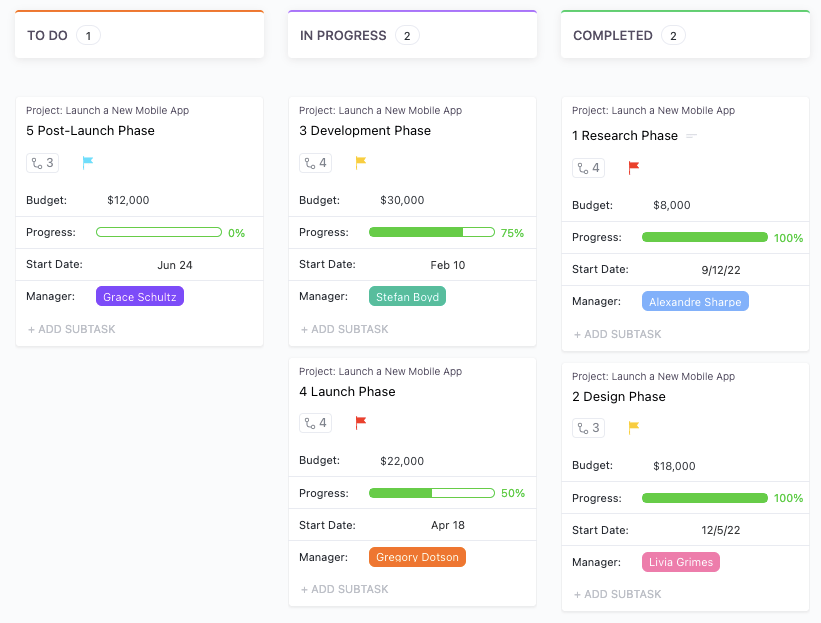
\includegraphics[width=0.9\linewidth]{Click_up.png}
    \caption{Exemplo kanban no ClickUp}
    \caption*{Fonte: \\ \url{https://clickup.com/blog/what-is-clickup-used-for/}}
    \label{fig:kanban-clickup}
\end{figure}
No ClickUp, você pode explorar sua carga de trabalho por meio de mais de 15 visualizações distintas, ajustadas para atender às suas demandas. Entre elas, destacam-se os formatos de Lista, Gantt, Linha do Tempo e o conhecido Kanban. Para uma visão geral do progresso dos projetos, os Painéis Ágeis entregam análises precisas e atualizadas em tempo real.
Os Dashboards do ClickUp são completamente adaptáveis, permitindo que sua equipe foque nas métricas e KPIs mais relevantes para os objetivos do projeto. Com mais de 100 formas de monitoramento, incluindo gráficos de burndown, queima, tempo de lead e ciclo, você pode acompanhar cada etapa dos projetos com máxima clareza e eficiência.

\clearpage

\begin{figure}[H]
    \centering
    \textbf{Quadro branco}\\[0.3cm]
    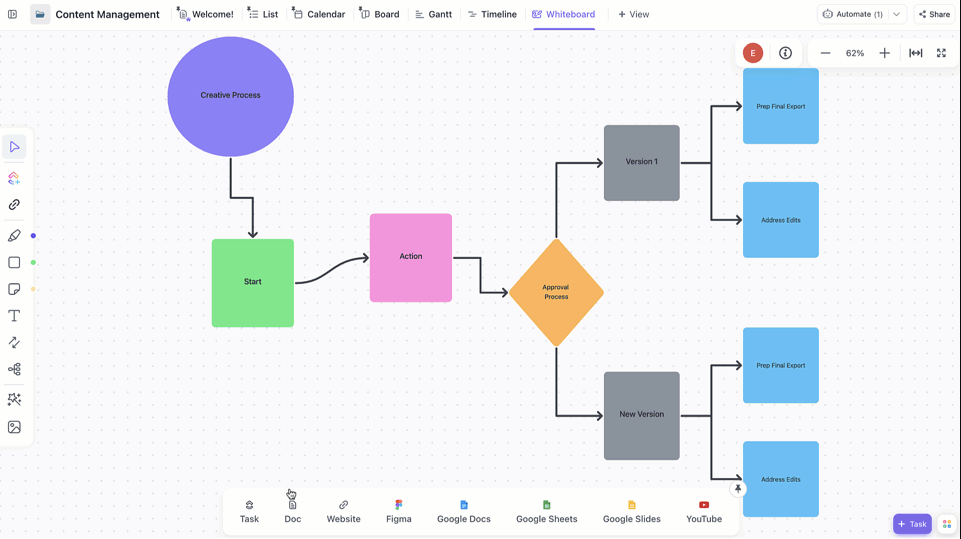
\includegraphics[width=0.9\linewidth]{quadro_branco.png}
    \caption{Fonte: \\ \url{https://clickup.com/blog/what-is-clickup-used-for/}}
    \label{fig:quadro-branco}
\end{figure}

Quadros brancos colaborativos: permitem brainstorm, planejamento e consolidação de ideias de forma visual, adicionando mídia e documentos.
\clearpage

\begin{figure}[H]
    \centering
    \textbf{ClickUp AI para uso de marketing, cronogramas, estratégia, notas de reuniões}\\[0.3cm]
    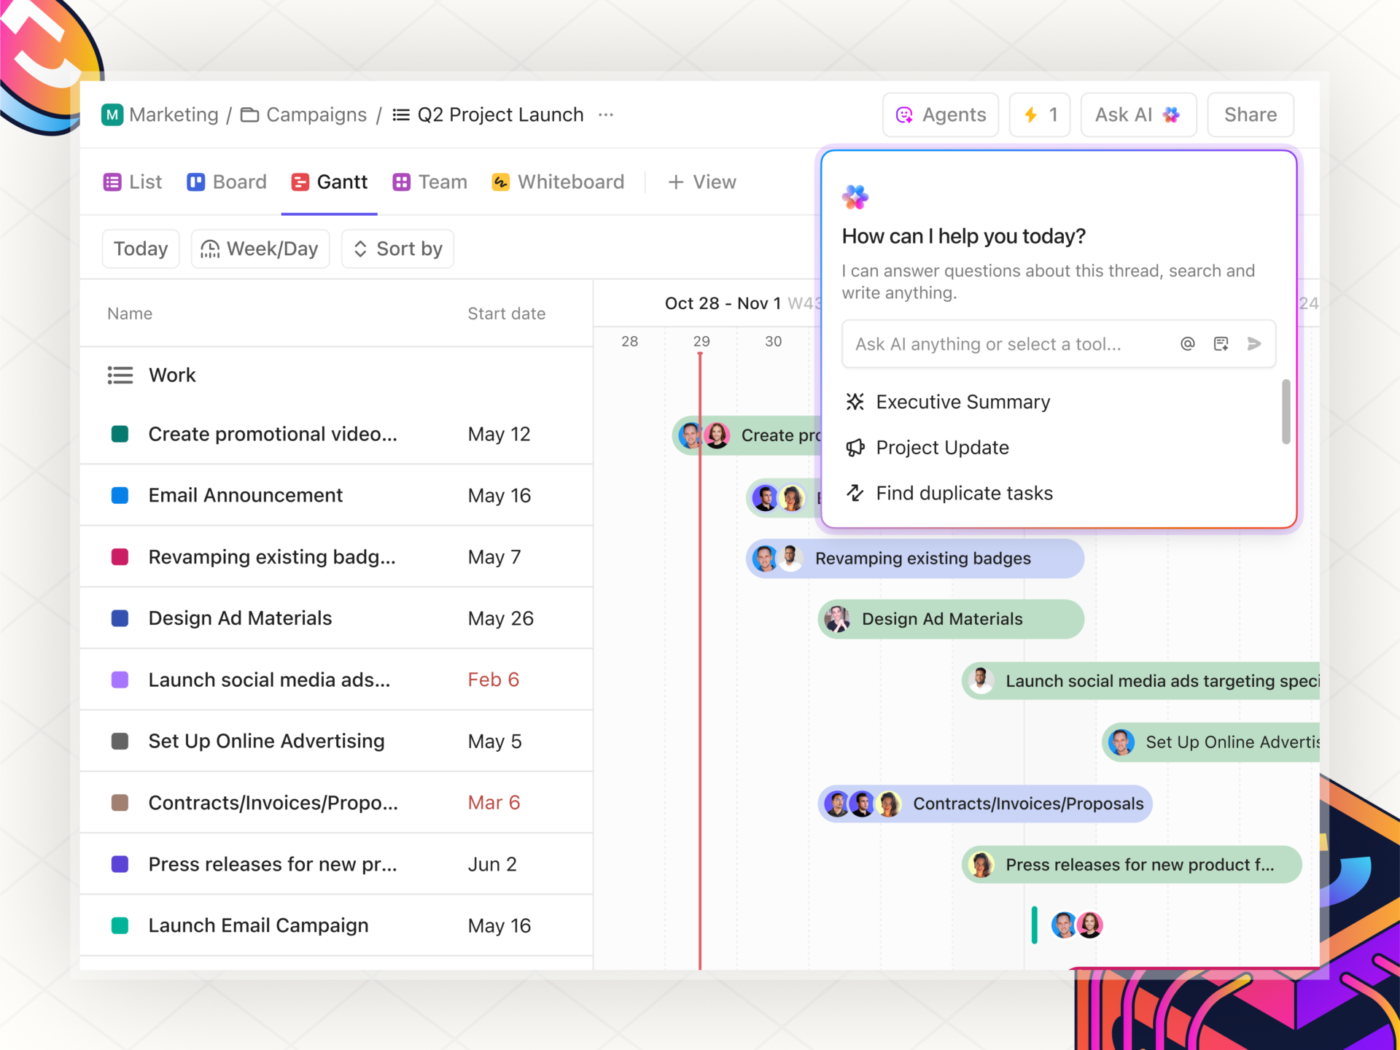
\includegraphics[width=0.9\linewidth]{ia2.png}
    \caption{Fonte: \\ \url{https://clickup.com/blog/how-to-execute-ai-marketing-campaigns/}}
    \label{fig:ia_clickup2}
\end{figure}

O ClickUp IA é uma ferramenta de produtividade que agiliza fluxos de trabalho, permitindo criar resumos de projetos, gerar novas tarefas e produzir conteúdos personalizados em segundos. Ele oferece prompts específicos para cada função, ajudando a organizar informações complexas e acelerar a execução das atividades diárias da equipe.
\clearpage

\subsection{Considerações Finais sobre o ClickUp}
O ClickUp oferece uma ampla gama de funcionalidades para diferentes tipos de projetos, sendo que muitos recursos não foram detalhados aqui. O que realmente se sobressai é sua versatilidade e alto grau de personalização. A plataforma possibilita que equipes de diversos tamanhos e áreas configurem o ambiente de trabalho conforme suas demandas, favorecendo a produtividade e a colaboração.
Além de ter a possibilidade de integrar a IA em praticamente todas as funções para agilizar o trabalho, como, por exemplo, criar tarefas, resumos, planos de ação, cronogramas, estratégias, notas de reuniões, entre outros.

\section{Análise Detalhada do Trello - Funcionamento, Vantagens e Limitações}
O Trello é a ferramenta de gestão de trabalho visual, criada com o intuito de capacitar os times para idealizar, planejar, administrar e celebrar o trabalho em conjunto de uma forma colaborativa, produtiva e organizada. Desenvolvido pela Atlassian em torno do método do quadro Kanban, ele
permite organizar as tarefas visualmente por meio de quadros, listas e cartões, facilitando a colaboração em equipe e a organização pessoal. No que diz respeito à acessibilidade, o Trello oferece a facilidade por meio de Android, sistema iOS, desktop, podendo ser utilizada na versão gratuita (Cintya Jíminni Brito da Silva, 2022).
Segundo Jaclyn McLean e Robin Canham (2018), Kanban é uma excelente filosofia para gerenciar o trabalho de forma flexível e garantir que os objetivos e prazos sejam cumpridos sem perder tempo em tarefas desnecessárias (também conhecido como "just in time").
Seu funcionamento se baseia na organização da informação em diferentes níveis:
\begin{itemize}
    \item \textbf{Dashboards/Quadros:} Eles representam um lugar para manter as informações, o que muitas vezes é necessário para projetos, times ou fluxos de trabalho grandes. Podem ser pessoais ou compartilhados com equipes
    \item \textbf{Listas:} Representam colunas dentro dos quadros, utilizadas para organizar tarefas em diferentes estágios, como “A Fazer”, “Em Andamento” e “Concluído”. Elas permitem criar um fluxo de trabalho visual, onde os cartões são movidos conforme avançam no processo, ou podem simplesmente servir como repositórios para ideias e informações.
    \item \textbf{Cartões:} São os itens dentro das listas que representam ideias e tarefas a realizar, são deslocados de uma coluna para outra em função do seu grau de progressão. Um cartão pode ser algo que precisa ser feito ou que precisa ser lembrado. Eles podem ser personalizados com descrições, datas de vencimento, rótulos, anexos e comentários.
    \item \textbf{Menu do quadro:} Localiza-se ao lado direito na tela do Trello e é a central de comando do quadro. Utiliza-se o menu para gerenciar permissões dos membros no quadro, controlar as configurações, pesquisar cartões, atribuir uma data de vencimento, ativar o recurso Power-Ups e criar automações.
    \item \textbf{Power-Ups:} Integração com Slack ou Microsoft Teams permite que comentários feitos no Trello geram notificações instantâneas, mantendo a equipe informada.
    \item \textbf{Checklist para sub-tarefas:} Cada cartão pode conter checklists para etapas menores de uma tarefa, garantindo que nada seja esquecido.
\end{itemize}

\subsection{Modelos Visuais do Trello no Método Kanban}
De acordo com Jaclyn McLean e Robin Canham(2018), uma vez que o Kanban foi escolhido para um projeto ou um conjunto de trabalho, e um quadro foi configurado, um indivíduo ou equipe pode criar um cartão para uma tarefa ou peça de trabalho individual e acompanhar
esse cartão através das diferentes listas, de a fazer, para fazendo, até feito.
A seguir, são apresentados alguns modelos visuais do Trello no método Kanban:
\begin{figure}[H]
    \begin{figure}[H]
        \centering
        \textbf{Exemplo de dashboard Trello versão gratuita}\\[0.3cm]
        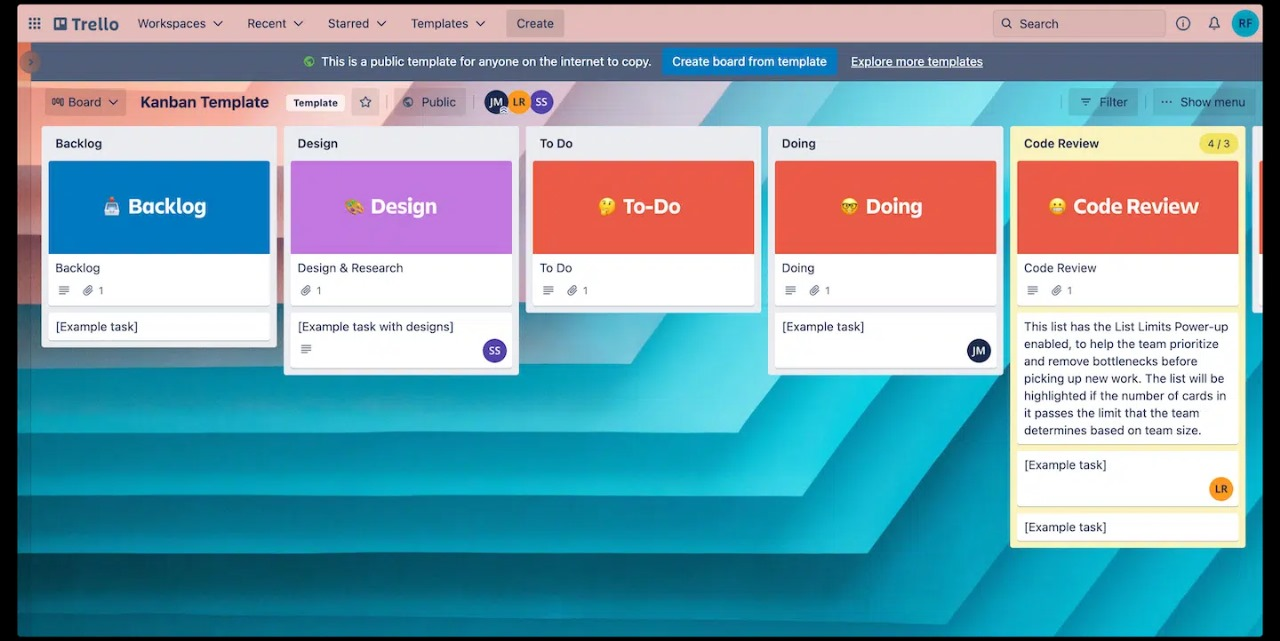
\includegraphics[width=0.9\linewidth]{luis1.jpg}
        % ---So tirar o 0.8 e mudar o exemple-image para o caminho real ---
        \caption{Fonte: \\ \url{https://salesdorado.com/pt-br/automacao/ferramentas-gerenciamento-projetos/avis-trello/}}
        \label{fig:kanban-trello-free}
    \end{figure}
\end{figure}
\clearpage

Embora o quadro Kanban esteja no centro do método Trello, a ferramenta dá acesso a outras formas de visualizar o fluxo de trabalho, disponíveis nos planos Premium pagos. Com isso, pode-se utilizar seu trabalho sob forma de uma linha do tempo, tabela, calendário, painel de controle e mapa.
\begin{figure}[H]
    \centering
    \textbf{Exemplo de dashboard Trello versão paga}\\[0.3cm]
    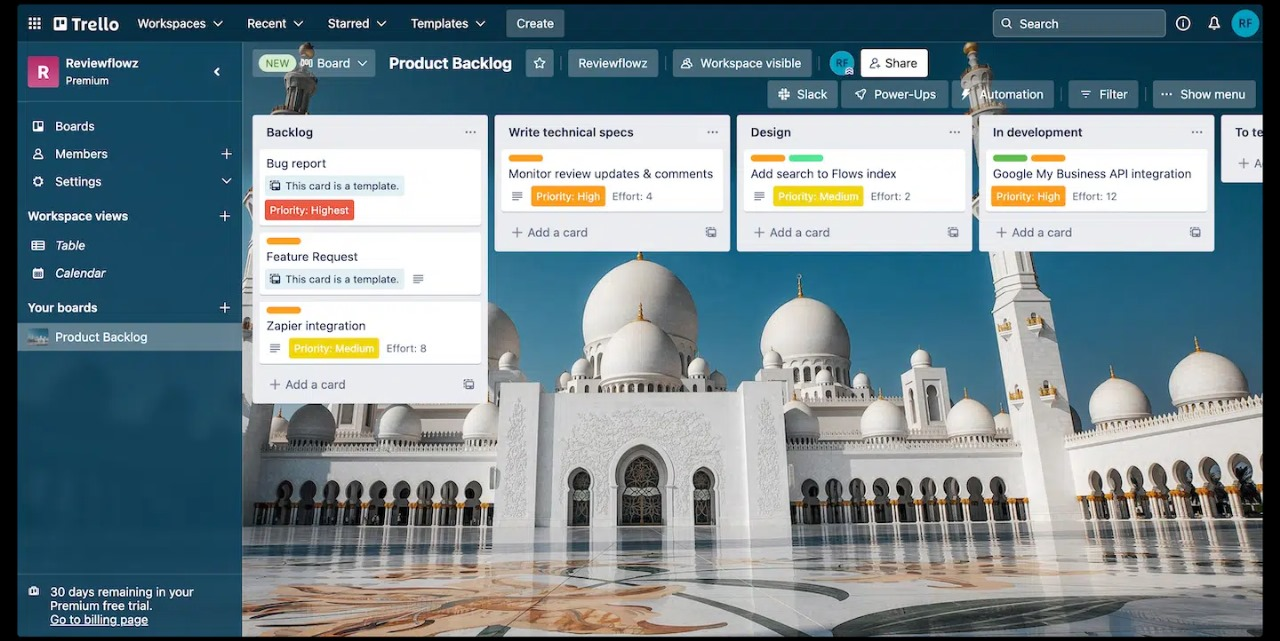
\includegraphics[width=0.9\linewidth]{luis2.jpg}
    \caption{Fonte: \\ \url{https://salesdorado.com/pt-br/automacao/ferramentas-gerenciamento-projetos/avis-trello/}}
    \label{fig:kanban-trello-pago}
\end{figure}

\begin{figure}[H]
    \centering
    \textbf{Exemplo de dashboard Trello versão paga}\\[0.3cm]
    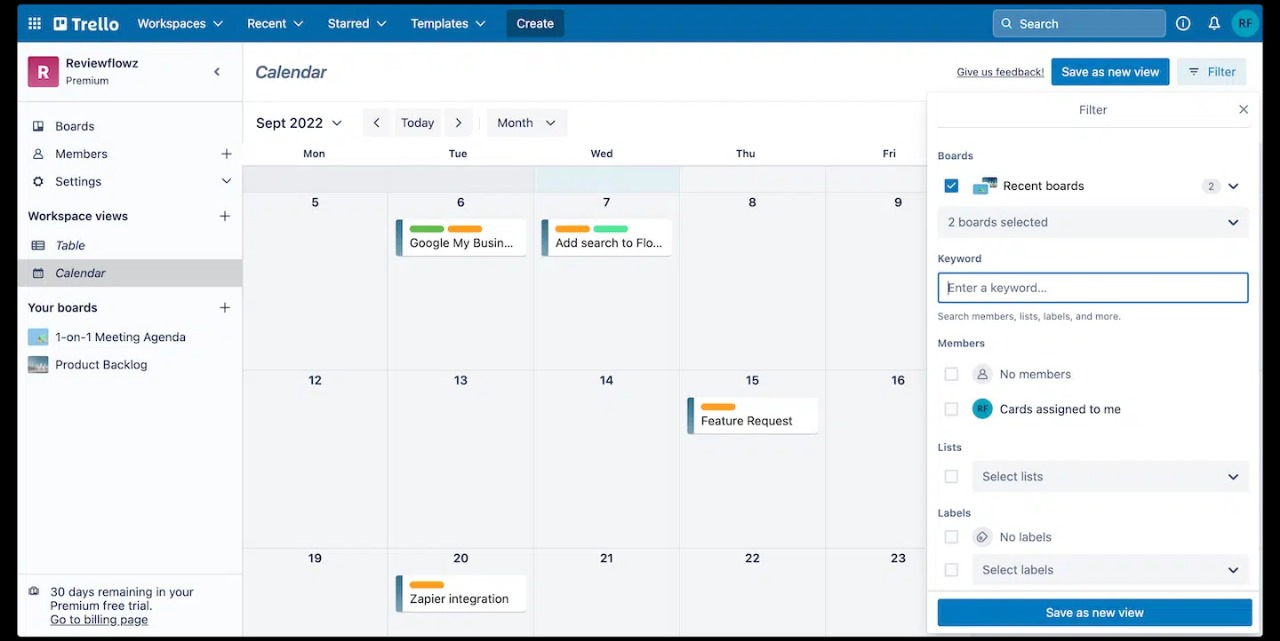
\includegraphics[width=0.9\linewidth]{luis3.jpg}
    \caption{Fonte: \\ \url{https://salesdorado.com/pt-br/automacao/ferramentas-gerenciamento-projetos/avis-trello/}}
    \label{fig:kanban-trello-pago-2}
\end{figure}
\clearpage

As visualizações da linha do tempo e do calendário permitem ver como o trabalho da equipe está organizado ao longo do tempo e antecipar os estrangulamentos. É possível também entrar na aba “tabela” e reunir mapas de diferentes tabelas em um único local para dar uma visão global sobre as criações.
\begin{figure}[H]
    \centering
    \textbf{Exemplo de dashboard Trello versão paga}\\[0.3cm]
    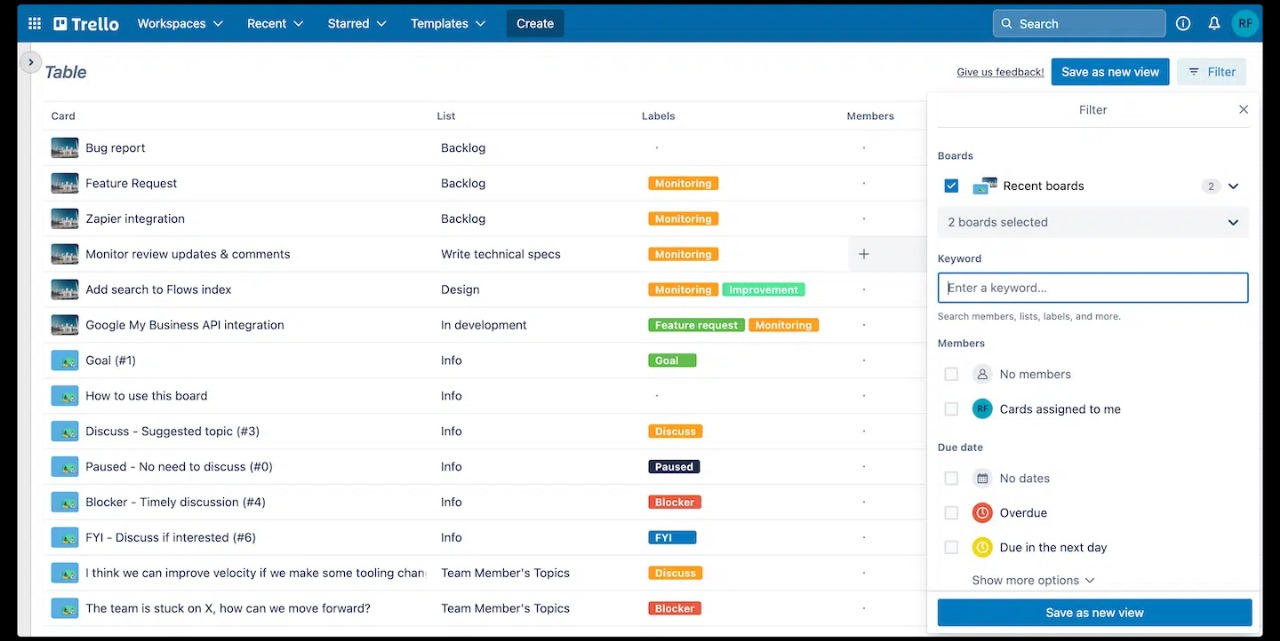
\includegraphics[width=0.9\linewidth]{luis4.jpg}
    \caption{Fonte: \\ \url{https://salesdorado.com/pt-br/automacao/ferramentas-gerenciamento-projetos/avis-trello/}}
    \label{fig:kanban-trello-pago-3}
\end{figure}

\section{Aprofundamento do Jira}

O Jira, desenvolvido pela Atlassian, consolidou-se como uma das principais plataformas para apoiar equipes ágeis que seguem metodologias como Scrum e Kanban. Sua adoção é ampla em equipes de desenvolvimento de software devido à sua robustez, flexibilidade e capacidade de integração com outras ferramentas, como o Confluence.

\subsection{Funcionalidades do Jira}
\begin{itemize}
    \item \textbf{Rastreabilidade de bugs e requisitos:} Cada problema ou história de usuário é registrado como uma issue, com histórico detalhado de alterações e comentários, facilitando o acompanhamento e a justificativa de decisões.
    \item \textbf{Sprints e boards:} Permite planejar ciclos de entrega, acompanhar o progresso em tempo real e realizar reuniões de alinhamento mais objetivas, seja por meio de boards Scrum ou Kanban.
    \item \textbf{Relatórios e métricas:} Fornece visibilidade sobre desempenho, produtividade e gargalos, com gráficos burndown, relatórios de sprint e dashboards customizáveis.
    \item \textbf{Integração com Confluence e outras ferramentas:} Possibilita centralização de documentação técnica e decisões, além de integração com sistemas de versionamento e automações.
\end{itemize}

Esses recursos tornam o Jira uma ferramenta robusta para apoiar tanto gestores quanto equipes técnicas, promovendo transparência e rastreabilidade em todo o ciclo de vida do projeto.

\subsection{Desafios de Comunicação em Projetos de TI}
A comunicação ineficiente em projetos de TI pode gerar atrasos, retrabalho e perda de qualidade. Entre os principais problemas estão:
\begin{itemize}
    \item Comunicação fragmentada: informações espalhadas em diferentes canais sem centralização.
    \item Falta de alinhamento entre equipe e gestores: objetivos e prazos mal comunicados.
    \item Pouca interação com o cliente: ausência de feedback estruturado.
    \item Perda de histórico de decisões: dificuldade em justificar escolhas sem registros formais.
\end{itemize}
O Jira ajuda a mitigar esses desafios ao centralizar dados e manter um histórico completo de atividades.

\subsection{Estratégias de Comunicação com Jira}
O Jira oferece diversas estratégias que fortalecem a comunicação organizacional:
\begin{itemize}
    \item Uso de boards Scrum e Kanban para alinhamento visual das tarefas.
    \item Comentários e menções dentro das issues, evitando dispersão da comunicação em e-mails.
    \item Relatórios de sprint para avaliação de progresso e pontos de melhoria.
    \item Integração com Confluence para documentação técnica e de reuniões.
    \item Notificações automáticas e dashboards para acompanhamento em tempo real.
\end{itemize}
Essas práticas contribuem para maior transparência, rastreabilidade e eficiência no trabalho em equipe.

\subsection{Exemplos Visuais: Kanban e Relatórios no Jira}
O Jira permite a visualização de tarefas por meio de quadros Kanban, que organizam atividades em colunas como ``A Fazer'', ``Em Andamento'' e ``Concluído''. Além disso, relatórios de sprint e gráficos burndown oferecem visão clara sobre desempenho e andamento das entregas.

\begin{figure}[H]
    \centering
    	\textbf{Exemplo de board Kanban no Jira}\\[0.3cm]
    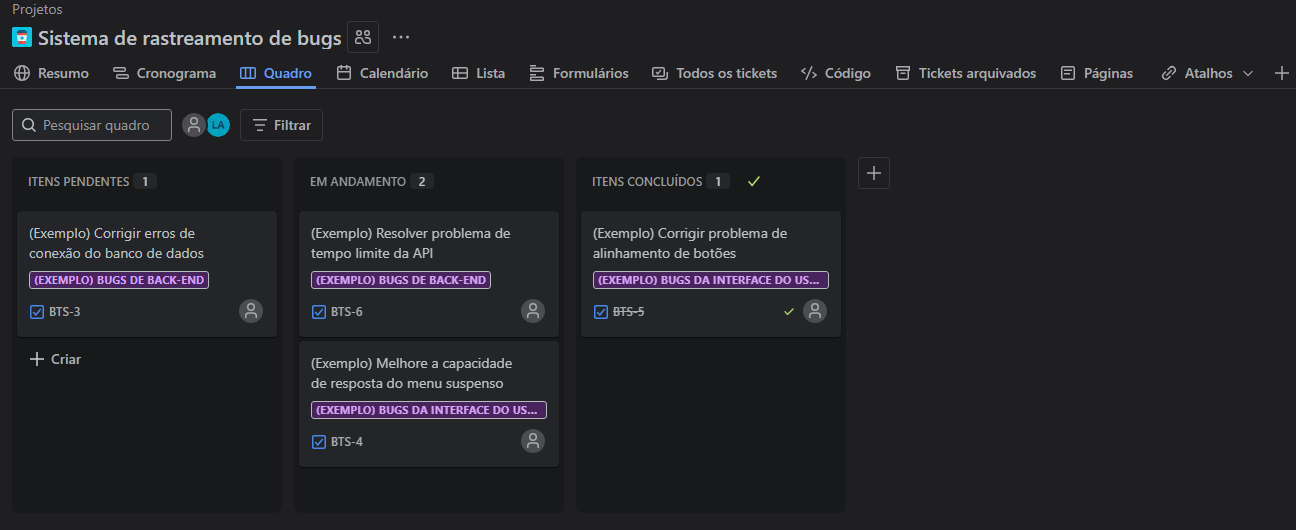
\includegraphics[width=0.9\linewidth]{jira_kanban.png}
    \caption{Fonte: Elaboração própria, (2025).}
    \label{fig:kanban-jira}
\end{figure}

\begin{figure}[H]
    \centering
    	\textbf{Exemplo de relatório de sprint no Jira}\\[0.3cm]
    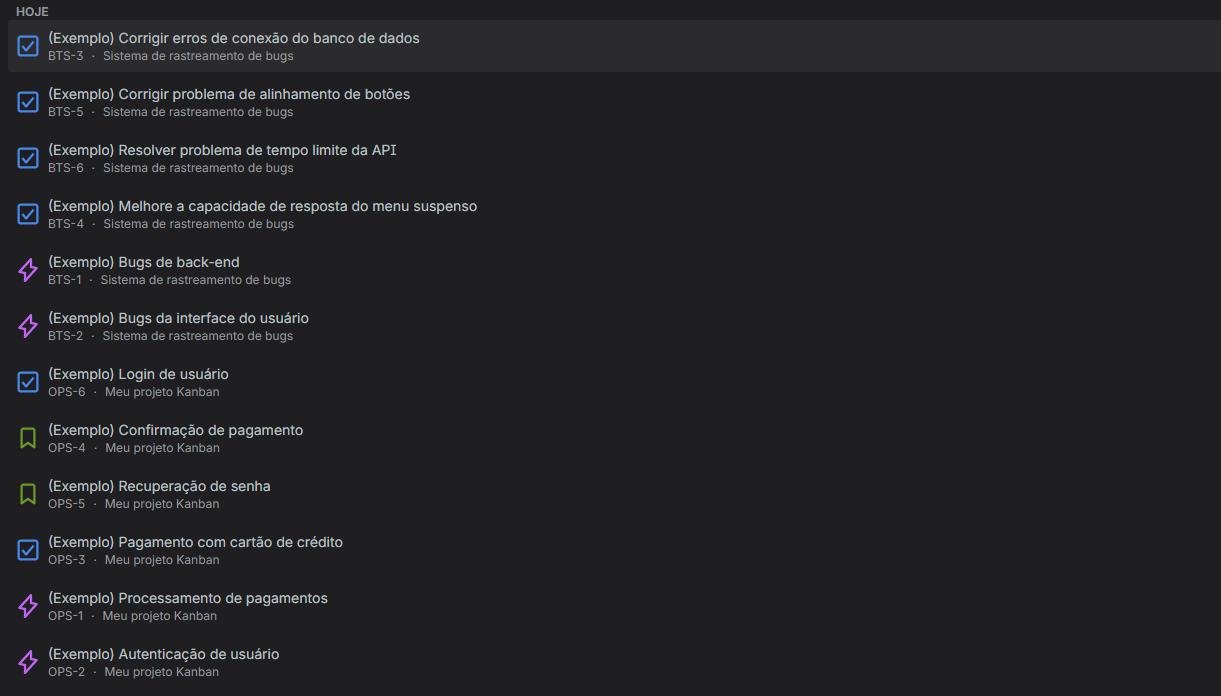
\includegraphics[width=0.9\linewidth]{relatorio.png}
    \caption{Fonte: Elaboração própria, (2025).}
    \label{fig:relatorio-jira}
\end{figure}


\clearpage
\subsection{Considerações Finais sobre o Jira}
O Jira é uma ferramenta estratégica para o gerenciamento de projetos de TI, especialmente em equipes ágeis. Sua capacidade de rastrear atividades, centralizar comunicação e integrar-se a outras plataformas fortalece a colaboração e reduz falhas de alinhamento. Quando utilizado de forma consciente, o Jira contribui para maior eficiência, transparência e qualidade na entrega de projetos tecnológicos.


\section{Conclusão}
Este estudo evidenciou que ferramentas modernas de gerenciamento de projetos, como ClickUp, Jira e Trello, oferecem funcionalidades que favorecem a comunicação, o acompanhamento de tarefas e a centralização de informações em equipes de TI. Cada plataforma apresenta pontos fortes específicos: o Jira se destaca em ambientes ágeis de grande porte pela rastreabilidade detalhada e integração com documentação, o Trello se sobressai pela simplicidade e visualização intuitiva de tarefas, e o ClickUp oferece uma solução integrada, combinando automações, dashboards e gerenciamento de documentos em um único espaço.

A escolha da ferramenta mais adequada depende de fatores como a maturidade da equipe, a complexidade do projeto e as necessidades de comunicação interna e externa. Além disso, a adoção de boas práticas de comunicação, aliada ao uso dessas ferramentas, contribui significativamente para a redução de falhas de alinhamento, duplicidade de tarefas e perda de histórico de decisões.

Portanto, o uso consciente e estratégico dessas plataformas pode promover maior eficiência, transparência e colaboração em projetos de Tecnologia da Informação, auxiliando gestores e equipes a alcançar melhores resultados.



\clearpage
\section*{Referências}

\begin{itemize}
    \item Project Management Institute. \textit{PMBOK Guide – A Guide to the Project Management Body of Knowledge}, 7th Edition, 2021.
    \item Schwaber, K. \textit{Agile Project Management with Scrum}. Microsoft Press, 2004.
    \item Sutherland, J.; Schwaber, K. \textit{The Scrum Guide}, 2020. Disponível em: \url{https://scrumguides.org/}.
    \item Wysocki, R. K. \textit{Effective Project Management: Traditional, Agile, Extreme}, 8th Edition, Wiley, 2019.
    \item Kerzner, H. \textit{Project Management: A Systems Approach to Planning, Scheduling, and Controlling}, 12th Edition, Wiley, 2017.

    \item \textbf{Documentação oficial das ferramentas:}
    \begin{itemize}
        \item ClickUp. ClickUp Help \& Docs. Disponível em: \url{https://docs.clickup.com/}. Acesso em: 22 ago. 2025.
        \item ClickUp. What is ClickUp used for? Disponível em: \url{https://clickup.com/blog/what-is-clickup-used-for/}. Acesso em: 7 set. 2025.
        \item Atlassian. Jira Software Guides. Disponível em: \url{https://www.atlassian.com/software/jira/guides}. Acesso em: 22 ago. 2025.
        \item Trello. Trello Guide. Disponível em: \url{https://trello.com/guide}. Acesso em: 22 ago. 2025.
    \end{itemize}
\end{itemize}
\end{document}
